\documentclass[class=article, crop=false]{standalone}
\usepackage{tikz}
\usepackage{subcaption}
\usetikzlibrary{calc}

\documentclass[class=article, crop=false]{standalone}
\usepackage{tikz}
\usepackage{subcaption}
\usetikzlibrary{calc}

\begin{document}
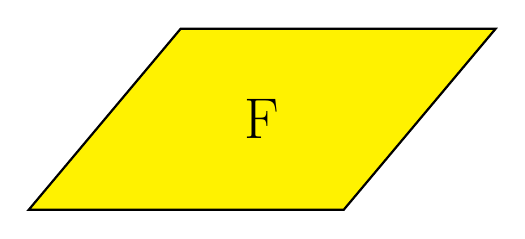
\begin{tikzpicture}
            % Define the lengths of the sides and the angle
            \def\a{4}  % length of side a
            \def\b{3}  % length of side b
            \def\angle{50}  % angle between sides a and b
        
            % Calculate the coordinates of the points
            \coordinate (A) at (0, 0);
            \coordinate (B) at (\a, 0);
            \coordinate (C) at ({\a + \b*cos(\angle)}, {\b * sin(\angle)});
            \coordinate (D) at ({\b * cos(\angle)}, {\b * sin(\angle)});

        
            % Draw the oblique unit cell
            \draw[thick,fill=yellow] (A) -- (B) -- (C) -- (D) -- cycle;
        
            \node at ($(A)!0.5!(C)$) {\huge F};
        \end{tikzpicture}
\end{document}
\end{document}